\documentclass[11pt]{scrartcl}
\usepackage[T1]{fontenc}
\usepackage[a4paper, left=3cm, right=2cm, top=2cm, bottom=2cm]{geometry}
\usepackage[activate]{pdfcprot}
\usepackage[ngerman]{babel}
\usepackage[parfill]{parskip}
\usepackage[utf8]{inputenc}
\usepackage[math]{kurier}
\usepackage{amsmath}
\usepackage{amssymb}
\usepackage{xcolor}
\usepackage{epstopdf}
\usepackage{txfonts}
\usepackage{fancyhdr}
\usepackage{graphicx}
\usepackage{prettyref}
\usepackage{hyperref}
\usepackage{eurosym}
\usepackage{setspace}
\usepackage{units}
\usepackage{eso-pic,graphicx}
\usepackage{icomma}
\usepackage{pdfpages}

\definecolor{darkblue}{rgb}{0,0,.5}
\hypersetup{pdftex=true, colorlinks=true, breaklinks=false, linkcolor=black, menucolor=black, urlcolor=darkblue}



\setlength{\columnsep}{2cm}


\newcommand{\arcsinh}{\mathrm{arcsinh}}
\newcommand{\asinh}{\mathrm{arcsinh}}
\newcommand{\ergebnis}{\textcolor{red}{\mathrm{Ergebnis}}}
\newcommand{\fehlt}{\textcolor{red}{Hier fehlen noch Inhalte.}}
\newcommand{\betanotice}{\textcolor{red}{Diese Aufgaben sind noch nicht in der Übung kontrolliert worden. Es sind lediglich meine Überlegungen und Lösungsansätze zu den Aufgaben. Es können Fehler enthalten sein!!! Das Dokument wird fortwährend aktualisiert und erst wenn das \textcolor{black}{beta} aus dem Dateinamen verschwindet ist es endgültig.}}
\newcommand{\half}{\frac{1}{2}}
\renewcommand{\d}{\, \mathrm d}
\newcommand{\punkte}{\textcolor{white}{xxxxx}}
\newcommand{\p}{\, \partial}
\newcommand{\dd}[1]{\item[#1] \hfill \\}

\renewcommand{\familydefault}{\sfdefault}
\renewcommand\thesection{}
\renewcommand\thesubsection{}
\renewcommand\thesubsubsection{}


\newcommand{\themodul}{Optische Technologie}
\newcommand{\thetutor}{Prof. Rateike}
\newcommand{\theuebung}{Klausur So15 Gedächtnisprotokoll}

\pagestyle{fancy}
\fancyhead[L]{\footnotesize{C. Hansen}}
\chead{\thepage}
\rhead{}
\lfoot{}
\cfoot{}
\rfoot{}

\title{\themodul{}, \theuebung{}, \thetutor}


\author{Christoph Hansen \\ {\small \href{mailto:chris@university-material.de}{chris@university-material.de}} }

\date{}


\begin{document}

\maketitle

Dieser Text ist unter dieser \href{http://creativecommons.org/licenses/by-nc-sa/4.0/}{Creative Commons} Lizenz veröffentlicht.

\textcolor{red}{Ich erhebe keinen Anspruch auf Vollständigkeit oder Richtigkeit. Falls ihr Fehler findet oder etwas fehlt, dann meldet euch bitte über den Emailkontakt.}

\tableofcontents


\newpage



\section{Aufgabe 1}



\section{Aufgabe 2 - Sphärische Abberation}

\subsection*{a}

Was ist die Ursache der shärischen Abberation?

\subsection*{b)}

?

\subsection*{c)}

Zeichnen sie den Strahlenverlauf durch eine Linse unter Berücksichtigung der sphärischen Abberation.

\subsection*{d)}

Was ist die älteste Methode um die sphärische Abberation zu korrigieren und was ist ihr Nachteil?

\subsection*{e)}

Gibt es heute bessere Methoden?


\section{Aufgabe 3 - Brechung}

Man hat ein \textbf{gleichseitiges} Glasdreieck, das von einem Lichtstrahl symetrisch durchlaufen wird. $n_{Glas} = 1,6$ und $n_{Luft} = 1$. Der Lichtstrahl fällt parallel zur Grundseite ein.


\begin{figure}[h]
	\centering
	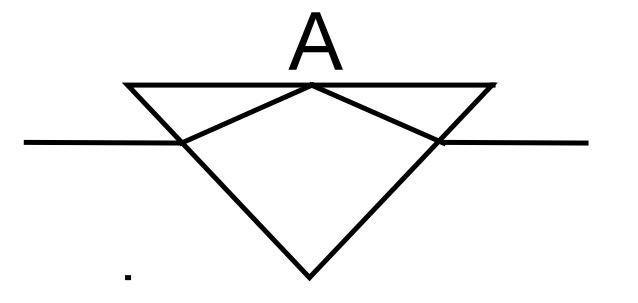
\includegraphics[scale=0.5]{A3_1.jpg}
	\caption{Skizze}
\end{figure}

\subsection*{a)}

Kommt es zur Totalreflexion, wenn sich an Punkt A Luft befindet?

\subsection*{b)}

Kommt es zur Totalreflexion, wenn sich an Punkt A Wasser ($n_{Wasser} = 1,334$) befindet?

\newpage

\section{Aufgabe 4 - Sterne und Teleskope}


Ein Stern hat den Durchmesser $\unit[2,38 \cdot 10^6]{km}$ und Abstand $\unit[8,6]{Lj}$.


\subsection*{a)}

Die Sterne nahe der Sonne haben alle die gleiche Größe, aber unterschiedliche Helligkeiten. Woran liegt das?


\subsection*{b)}

Du hast ein Teleskop dessen Linse eine Brennweite $\unit[25]{m}$ beträgt. Berechne die Bildgröße des Sterns.


\subsection*{c)}

??

\section{Aufgabe 5 - Besselversuch}

Alles zum Besselversuch. Aufbau, Funktion, Methode, Berechnung der Brennweite der vermessenen Linse.





















\end{document}